% The generic preamble
\documentclass[10pt,letterpaper,fleqn,titlepage]{article}

% Define packages to use
\usepackage{natbib}
\usepackage[dvips]{graphicx,color}
\usepackage{amsmath,amssymb}
\usepackage{bm}
\usepackage{caption}
\usepackage{xr}
\usepackage{ifthen}
\usepackage[dvipdfm,colorlinks,linkcolor=blue,citecolor=blue,urlcolor=blue]{hyperref}
\usepackage{fancybox}
\usepackage{textcomp}
\usepackage{alltt}
%\usepackage{floatflt}
%\usepackage{svn}


% Redefine default page
\setlength{\textheight}{9in}  % 1" above and below
\setlength{\textwidth}{6.75in}   % 0.5" left and right
\setlength{\oddsidemargin}{-0.25in}

% Redefine default paragraph
\setlength{\parindent}{0pt}
\setlength{\parskip}{1ex plus 0.5ex minus 0.2ex}

% Define caption width and default fonts
\setlength{\captionmargin}{0.5in}
\renewcommand{\captionfont}{\sffamily}
\renewcommand{\captionlabelfont}{\bfseries\sffamily}

% Define commands for super- and subscript in text mode
\newcommand{\superscript}[1]{\ensuremath{^\textrm{#1}}}
\newcommand{\subscript}[1]{\ensuremath{_\textrm{#1}}}

% Derived commands
\newcommand{\invcm}{\textrm{cm\superscript{-1}}}
\newcommand{\micron}{\ensuremath{\mu\textrm{m}}}

\newcommand{\df}{\ensuremath{\delta f}}
\newcommand{\Df}{\ensuremath{\Delta f}}
\newcommand{\dx}{\ensuremath{\delta x}}
\newcommand{\Dx}{\ensuremath{X_{max}}}
\newcommand{\Xeff}{\ensuremath{X_{eff}}}

\newcommand{\water}{\textrm{H\subscript{2}O}}
\newcommand{\carbondioxide}{\textrm{CO\subscript{2}}}
\newcommand{\ozone}{\textrm{O\subscript{3}}}

\newcommand{\taup}[1]{\ensuremath{\tau_{#1}}}
\newcommand{\efftaup}[1]{\ensuremath{\tau_{#1}^{*}}}

\newcommand{\textbfm}[1]{\boldmath\ensuremath{#1}\unboldmath}

\newcommand{\rb}[1]{\raisebox{1.5ex}[0pt]{#1}}

\newcommand{\f}[1]{\texttt{#1}}

% Define how equations are numbered
\numberwithin{equation}{section}
\numberwithin{figure}{section}
\numberwithin{table}{section}

% Define a command for title page author email footnote
\newcommand{\email}[1]
{%
  \renewcommand{\thefootnote}{\alph{footnote}}%
  \footnote{#1}
  \renewcommand{\thefootnote}{\arabic{footnote}}
}

% Define a command to print the Office Note subheading
\newcommand{\notesubheading}[1]
{%
  \ifthenelse{\equal{#1}{}}{}
  { {\Large\bfseries Office Note #1\par}%
    {\scriptsize \sc This is an unreviewed manuscript, primarily intended for informal}\\ 
    {\scriptsize \sc exchange of information among JCSDA researchers\par}%
  }
}

% Redefine the maketitle macro
\makeatletter
\def\docseries#1{\def\@docseries{#1}}
\def\docnumber#1{\def\@docnumber{#1}}
\renewcommand{\maketitle}
{%
  \thispagestyle{empty}
  \vspace*{1in}
  \begin{center}%
     \sffamily
     {\huge\bfseries Joint Center for Satellite Data Assimilation\par}%
     \notesubheading{\@docnumber}
  \end{center}
  \begin{flushleft}%
     \sffamily
     \vspace*{0.5in}
     {\Large\bfseries\ifthenelse{\equal{\@docseries}{}}{}{\@docseries: }\@title\par}%
     \medskip
     {\large\@author\par}%
     \medskip
     {\large\@date\par}%
     \bigskip\hrule\vspace*{2pc}%
  \end{flushleft}%
  \newpage
  \setcounter{footnote}{0}
}
\makeatother
\docseries{}
\docnumber{}


% Define a command for a DRAFT watermark
\usepackage{eso-pic}
\newcommand{\draftwatermark}
{
  \AddToShipoutPicture{%
    \definecolor{lightgray}{gray}{.85}
    \setlength{\unitlength}{1in}
    \put(2.5,3.5){%
      \rotatebox{45}{%
        \resizebox{4in}{1in}{%
          \textsf{\textcolor{lightgray}{DRAFT}}
        }
      }
    }
  }
}




% Title info
\title{GOES-14 and -15 Sounder Spectral Response Functions}
\author{Paul van Delst\email{paul.vandelst@noaa.gov}\\JCSDA/EMC/SAIC\\[0.25in]
        David Groff\email{david.groff@noaa.gov}\\JCSDA/EMC/SAIC}
\date{September, 2008}
\docnumber{(unassigned)}
\docseries{CRTM}


%-------------------------------------------------------------------------------
%                            Ze document begins...
%-------------------------------------------------------------------------------
\begin{document}
\maketitle

%\draftwatermark


\section{Introduction}
%=====================
This document displays the spectral response functions (SRFs) of the GOES-0(14) and -P(15) sounder instrument, obtained from http://cimss.ssec.wisc.edu/goes/calibration/SRF. These SRFs will be used to generate instrument resolution transmtitances and, from those, transmittance model coefficients for use in the CRTM.


\section{GOES-O(14) Sounder SRFs}
%================================

\subsection{Nominal SRF plots}
%-----------------------------
Plots of the SRF data for each channel detector, along with the detector average, are shown for channels 1-6 in figure \ref{fig:sndr_g14.ch1-6}, channels 7-12 in figure \ref{fig:sndr_g14.ch7-12}, and channels 13-18 in figure \ref{fig:sndr_g14.ch13-18}.

\begin{figure}[htp]
  \centering
  \begin{tabular}{c c}
    \includegraphics[scale=0.5]{graphics/nominal/sndr_g14.ch1.srf.eps} &
    \includegraphics[scale=0.5]{graphics/nominal/sndr_g14.ch2.srf.eps} \\
    \includegraphics[scale=0.5]{graphics/nominal/sndr_g14.ch3.srf.eps} &
    \includegraphics[scale=0.5]{graphics/nominal/sndr_g14.ch4.srf.eps} \\
    \includegraphics[scale=0.5]{graphics/nominal/sndr_g14.ch5.srf.eps} &
    \includegraphics[scale=0.5]{graphics/nominal/sndr_g14.ch6.srf.eps}
  \end{tabular}
  \caption{GOES-O(14) Sounder SRF for channels 1 to 6.}
  \label{fig:sndr_g14.ch1-6}
\end{figure}

\begin{figure}[htp]
  \centering
  \begin{tabular}{c c}
    \includegraphics[scale=0.5]{graphics/nominal/sndr_g14.ch7.srf.eps} &
    \includegraphics[scale=0.5]{graphics/nominal/sndr_g14.ch8.srf.eps} \\
    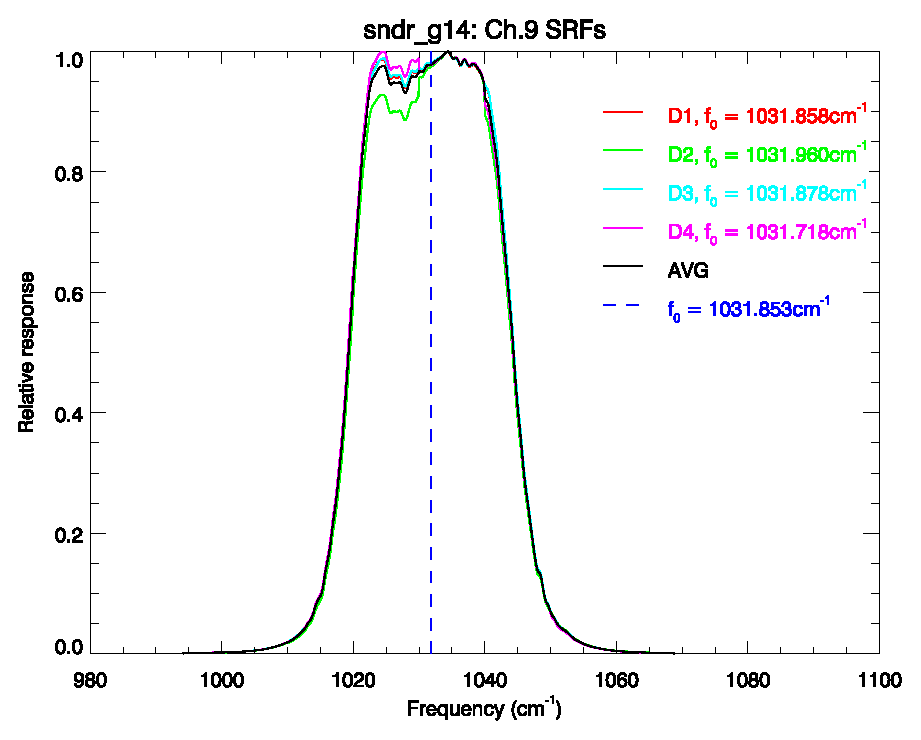
\includegraphics[scale=0.5]{graphics/nominal/sndr_g14.ch9.srf.eps} &
    \includegraphics[scale=0.5]{graphics/nominal/sndr_g14.ch10.srf.eps} \\
    \includegraphics[scale=0.5]{graphics/nominal/sndr_g14.ch11.srf.eps} &
    \includegraphics[scale=0.5]{graphics/nominal/sndr_g14.ch12.srf.eps}
  \end{tabular}
  \caption{GOES-O(14) Sounder SRF for channels 7 to 12.}
  \label{fig:sndr_g14.ch7-12}
\end{figure}

\begin{figure}[htp]
  \centering
  \begin{tabular}{c c}
    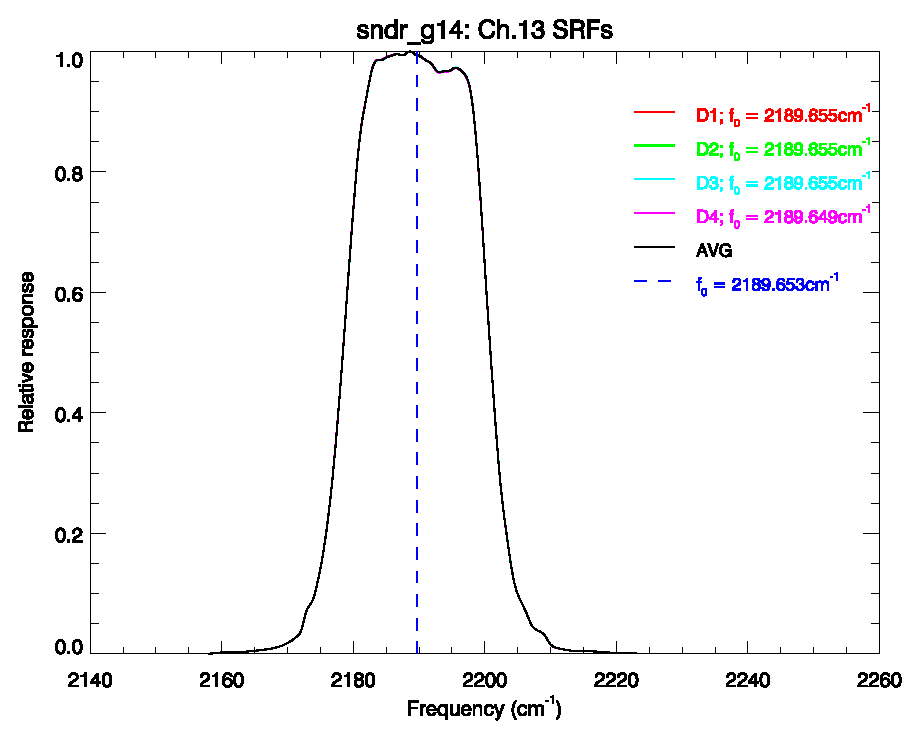
\includegraphics[scale=0.5]{graphics/nominal/sndr_g14.ch13.srf.eps} &
    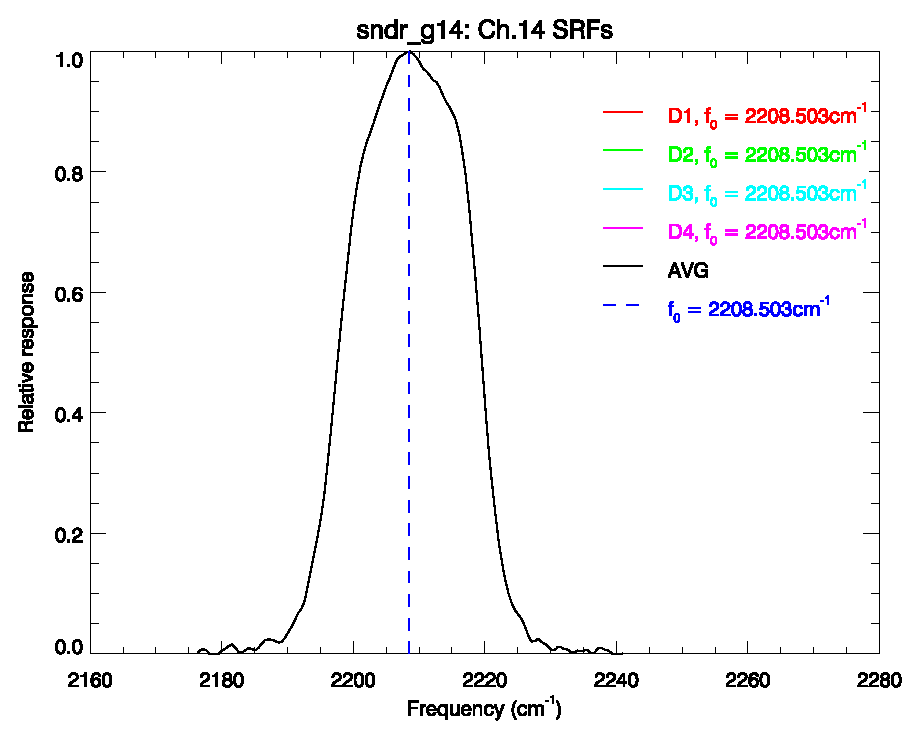
\includegraphics[scale=0.5]{graphics/nominal/sndr_g14.ch14.srf.eps} \\
    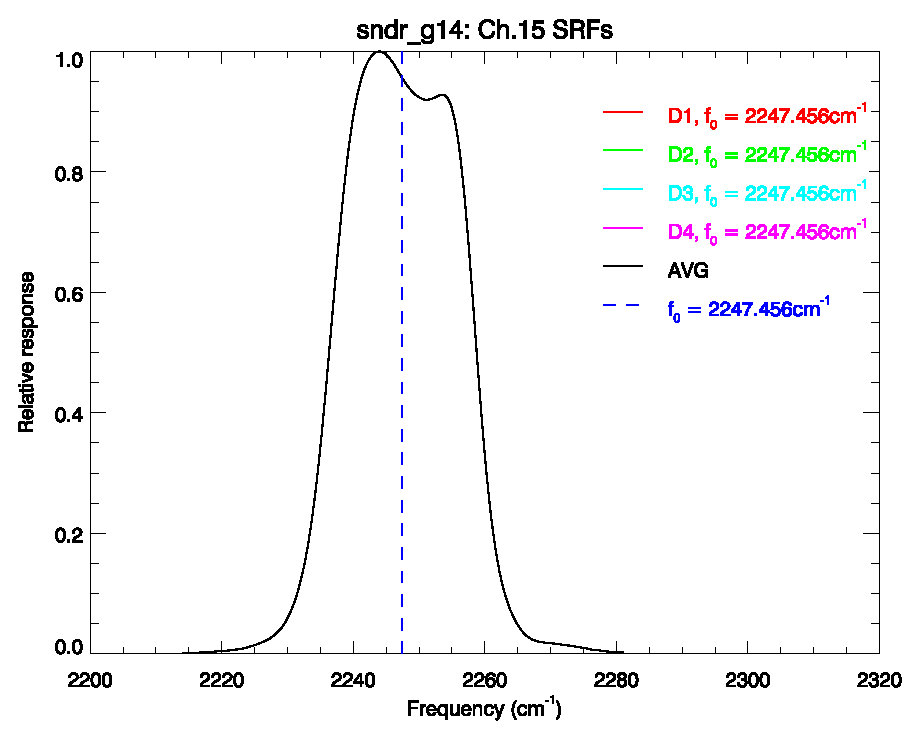
\includegraphics[scale=0.5]{graphics/nominal/sndr_g14.ch15.srf.eps} &
    \includegraphics[scale=0.5]{graphics/nominal/sndr_g14.ch16.srf.eps} \\
    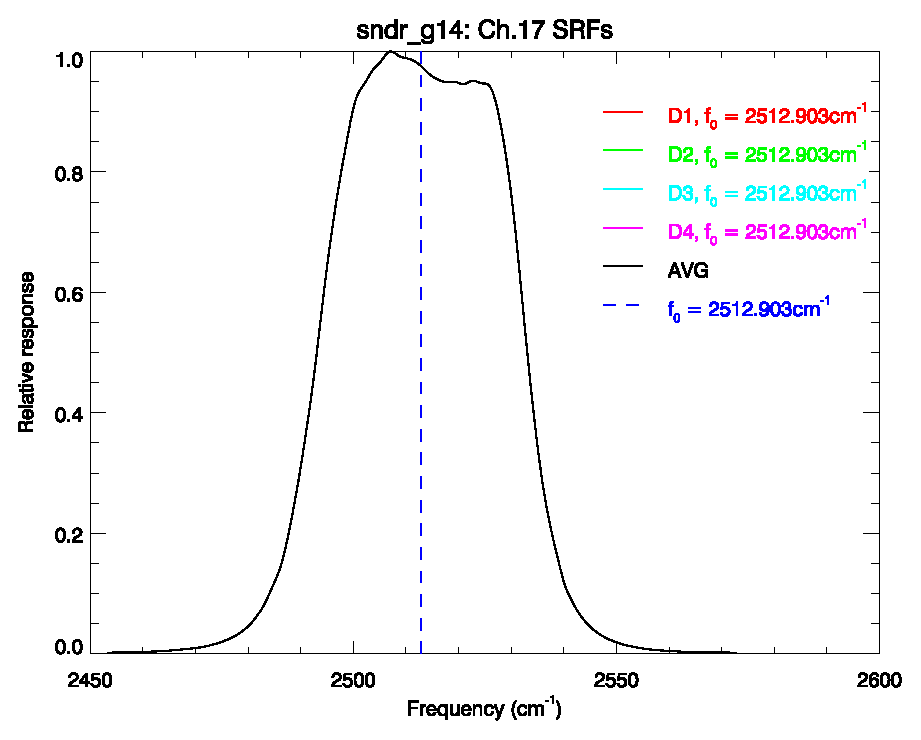
\includegraphics[scale=0.5]{graphics/nominal/sndr_g14.ch17.srf.eps} &
    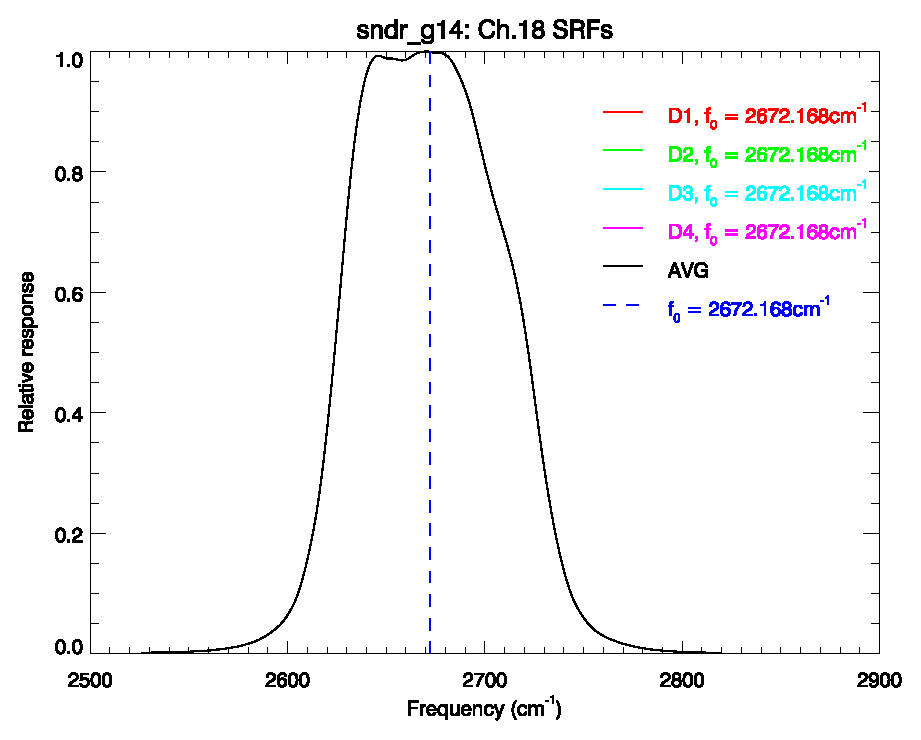
\includegraphics[scale=0.5]{graphics/nominal/sndr_g14.ch18.srf.eps}
  \end{tabular}
  \caption{GOES-O(14) Sounder SRF for channels 13 to 18.}
  \label{fig:sndr_g14.ch13-18}
\end{figure}

\subsection{Anomalous Features}
%------------------------------
Closer inspection of the GOES-0(14) sounder SRFs showed both ambiguous and clear anomalies for several channels. Magnifications of the SRF plots for the suspect channels are shown in figure \ref{fig:sndr_g14.zoom_anomaly}. The anomalies are
\begin{description}
  \item[Ch.5] The begin point of this channel is unlike any others in that it starts at a relatively large value. Was the begin point of the actual measurements somehow truncated, or is this feature an artifact of fitting the measurements?
  \item[Ch.6] The negative values for the low-frequency beginning portions of this SRF have been truncated. The shape of the remaining positive data begs the question: are these data real or an artifact of the fitting algorithm (high order polynomial or spline)?
  \item[Ch.9] There are clear, and for 1030\invcm{} quite large, discontinuities in the data.
  \item[Ch.10] Again, discontinuities in the SRFs are evident. Here they clearly occur every 10\invcm{}.
  \item[Ch.11] Discontinuities at 10\invcm{} intervals.
  \item[Ch.12] Discontinuities at 10\invcm{} intervals.
\end{description}

\begin{figure}[htp]
  \centering
  \begin{tabular}{c c}
    \hspace{1.0em}\textsf{High begin point value} &
    \textsf{Negative truncation. Are positive values a fit artifact?} \\
    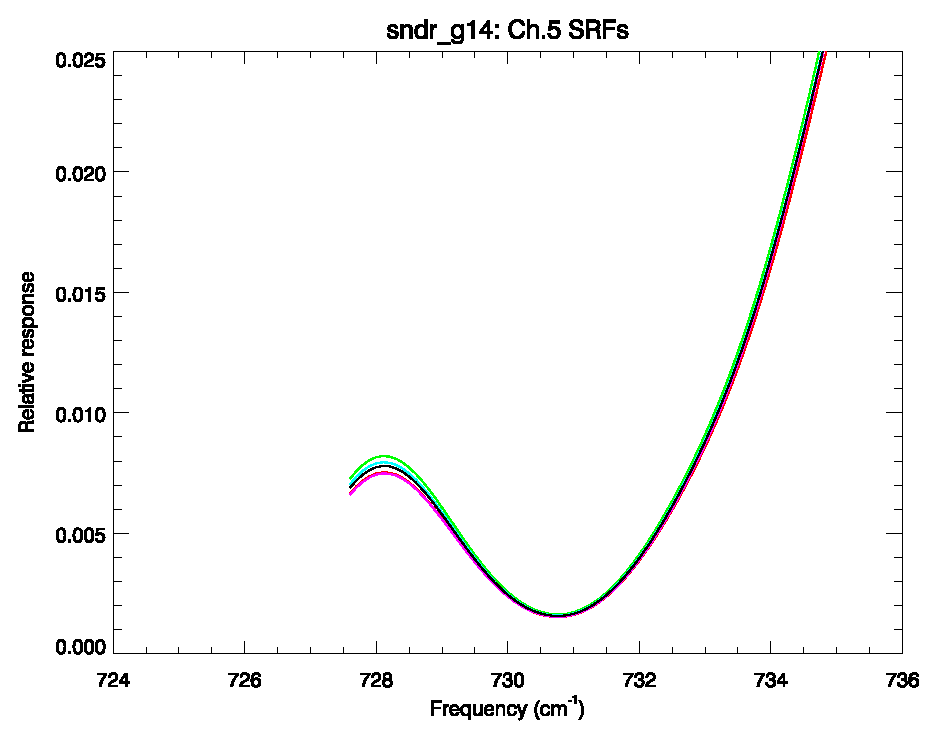
\includegraphics[scale=0.5]{graphics/zoom_anomaly/sndr_g14.ch5.srf.eps} &
    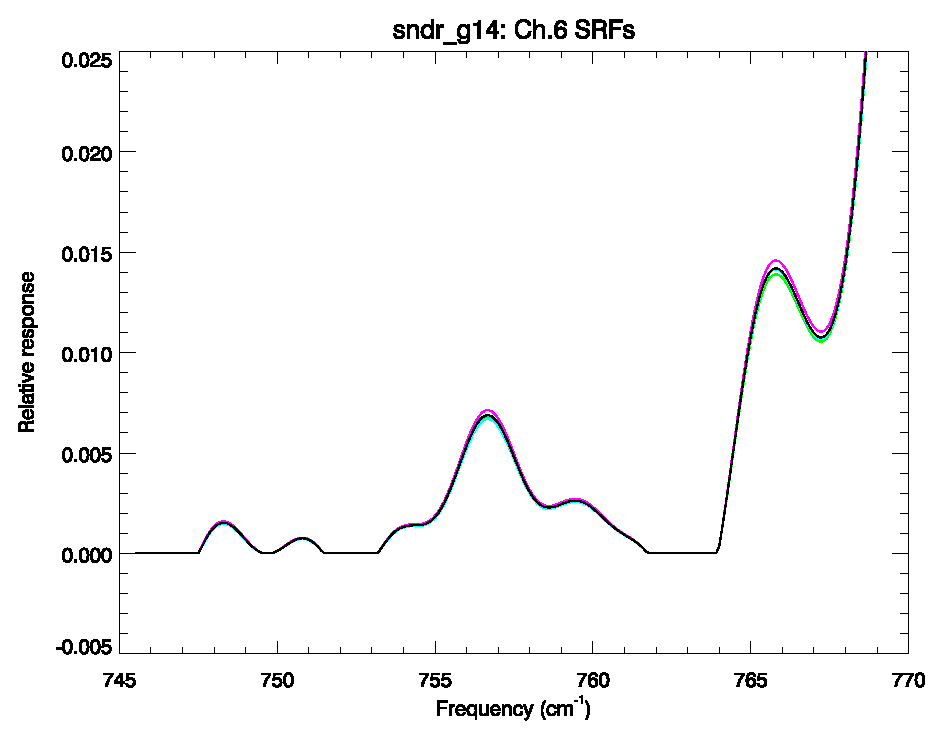
\includegraphics[scale=0.5]{graphics/zoom_anomaly/sndr_g14.ch6.srf.eps} \\\\
    \hspace{1.0em}\textsf{Discontinuities at 1030 and 1040cm$^{-1}$} &
    \hspace{1.0em}\textsf{Discontinuities at 1340, 1350, and 1360cm$^{-1}$.} \\
    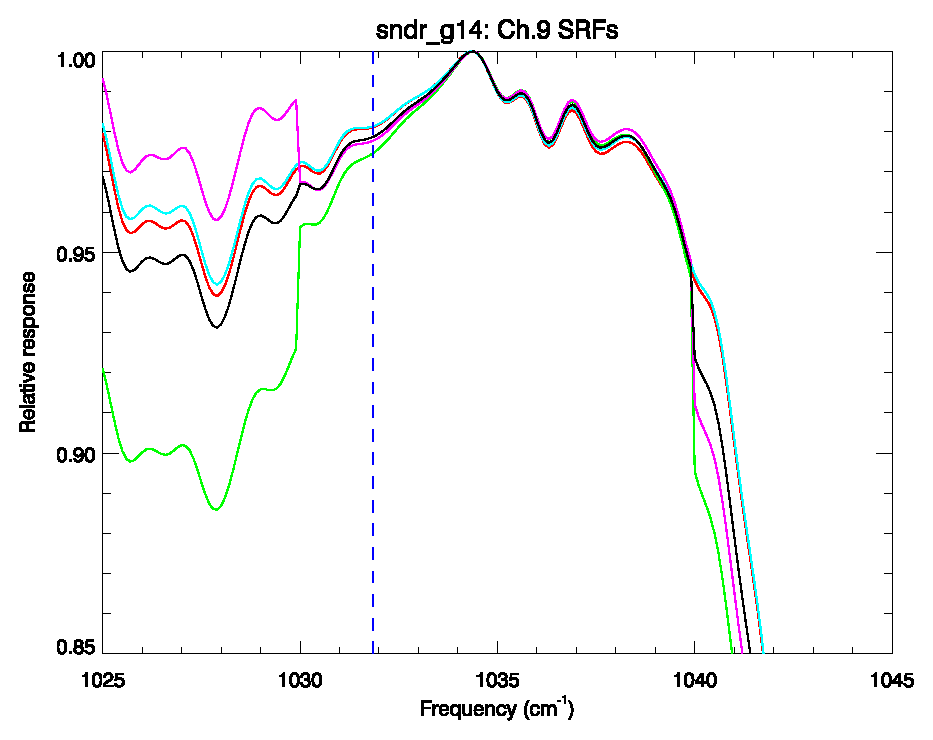
\includegraphics[scale=0.5]{graphics/zoom_anomaly/sndr_g14.ch9.srf.eps} &
    \includegraphics[scale=0.5]{graphics/zoom_anomaly/sndr_g14.ch10.srf.eps} \\\\
    \hspace{1.0em}\textsf{Discontinuities at 1410, 1420, and 1430cm$^{-1}$.} &
    \hspace{1.0em}\textsf{Discontinuities every 10cm$^{-1}$.} \\
    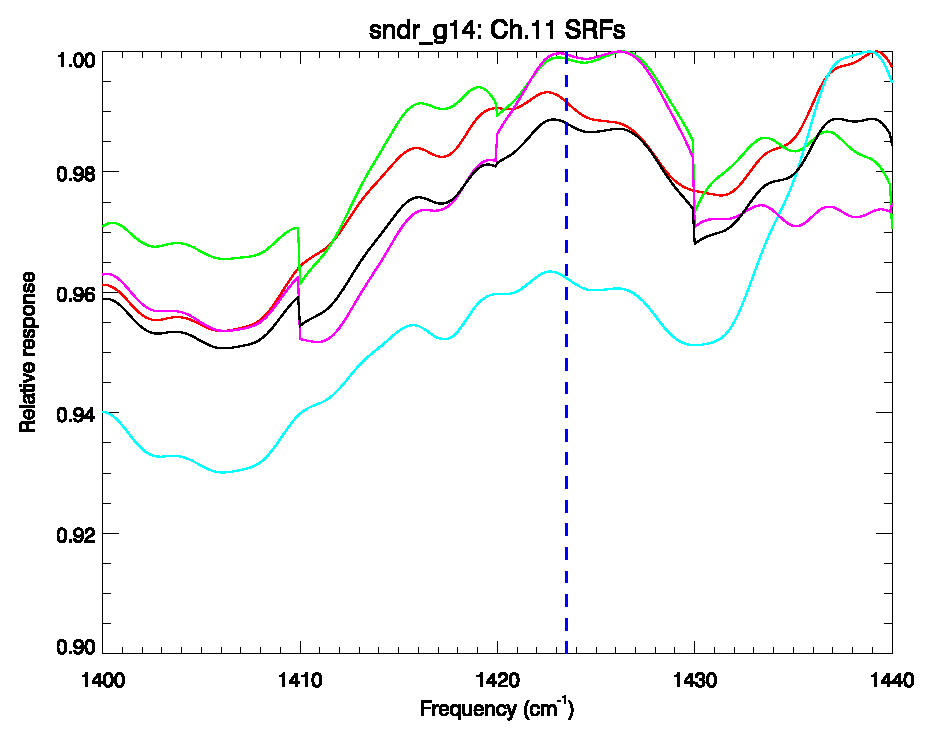
\includegraphics[scale=0.5]{graphics/zoom_anomaly/sndr_g14.ch11.srf.eps} &
    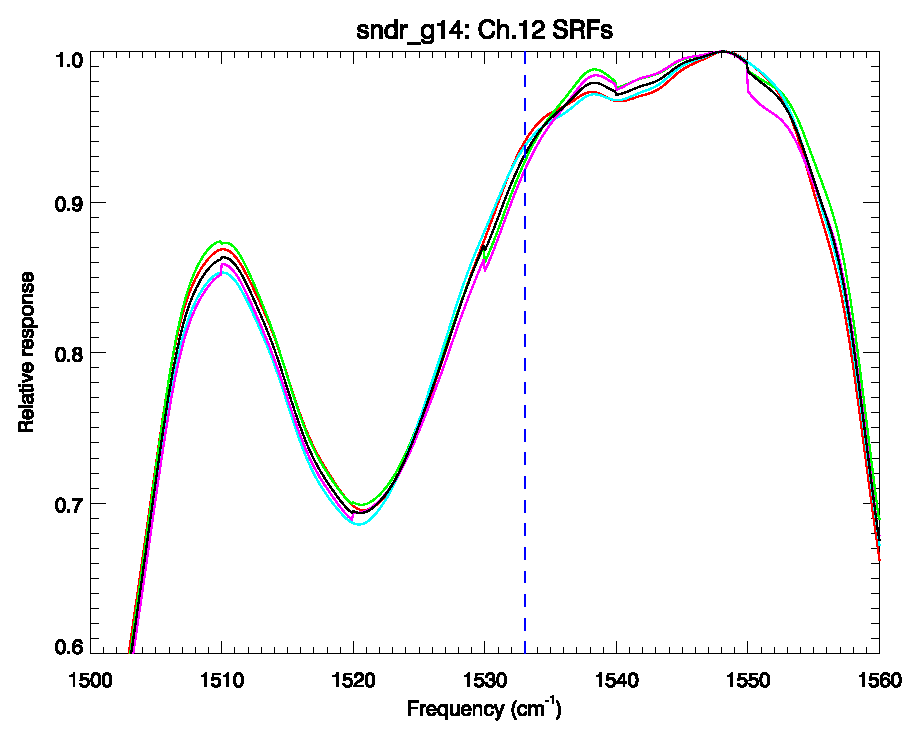
\includegraphics[scale=0.5]{graphics/zoom_anomaly/sndr_g14.ch12.srf.eps}
  \end{tabular}
  \caption{Magnification of GOES-O(14) Sounder SRFs for channels 5, 6, 9, 10, 11, and 12; indicating possible data anomalies. Detector and average plot colours are the same as for previous figures.}
  \label{fig:sndr_g14.zoom_anomaly}
\end{figure}




\section{GOES-P(15) Sounder SRFs}
%================================
Plots of the SRF data for each channel detector, along with the detector average, are shown for channels 1-6 in figure \ref{fig:sndr_g15.ch1-6}, channels 7-12 in figure \ref{fig:sndr_g15.ch7-12}, and channels 13-18 in figure \ref{fig:sndr_g15.ch13-18}.


\subsection{Nominal SRF plots}
%-----------------------------

\begin{figure}[htp]
  \centering
  \begin{tabular}{c c}
    \includegraphics[scale=0.5]{graphics/nominal/sndr_g15.ch1.srf.eps} &
    \includegraphics[scale=0.5]{graphics/nominal/sndr_g15.ch2.srf.eps} \\
    \includegraphics[scale=0.5]{graphics/nominal/sndr_g15.ch3.srf.eps} &
    \includegraphics[scale=0.5]{graphics/nominal/sndr_g15.ch4.srf.eps} \\
    \includegraphics[scale=0.5]{graphics/nominal/sndr_g15.ch5.srf.eps} &
    \includegraphics[scale=0.5]{graphics/nominal/sndr_g15.ch6.srf.eps}
  \end{tabular}
  \caption{GOES-P(15) Sounder SRF for channels 1 to 6.}
  \label{fig:sndr_g15.ch1-6}
\end{figure}

\begin{figure}[htp]
  \centering
  \begin{tabular}{c c}
    \includegraphics[scale=0.5]{graphics/nominal/sndr_g15.ch7.srf.eps} &
    \includegraphics[scale=0.5]{graphics/nominal/sndr_g15.ch8.srf.eps} \\
    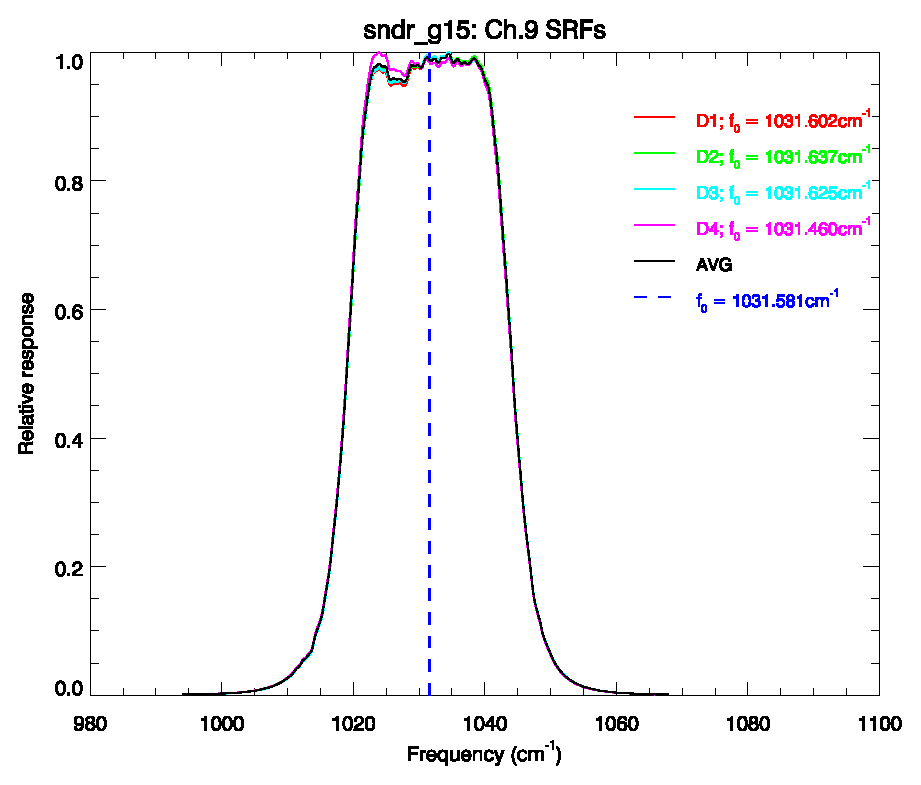
\includegraphics[scale=0.5]{graphics/nominal/sndr_g15.ch9.srf.eps} &
    \includegraphics[scale=0.5]{graphics/nominal/sndr_g15.ch10.srf.eps} \\
    \includegraphics[scale=0.5]{graphics/nominal/sndr_g15.ch11.srf.eps} &
    \includegraphics[scale=0.5]{graphics/nominal/sndr_g15.ch12.srf.eps}
  \end{tabular}
  \caption{GOES-P(15) Sounder SRF for channels 7 to 12.}
  \label{fig:sndr_g15.ch7-12}
\end{figure}

\begin{figure}[htp]
  \centering
  \begin{tabular}{c c}
    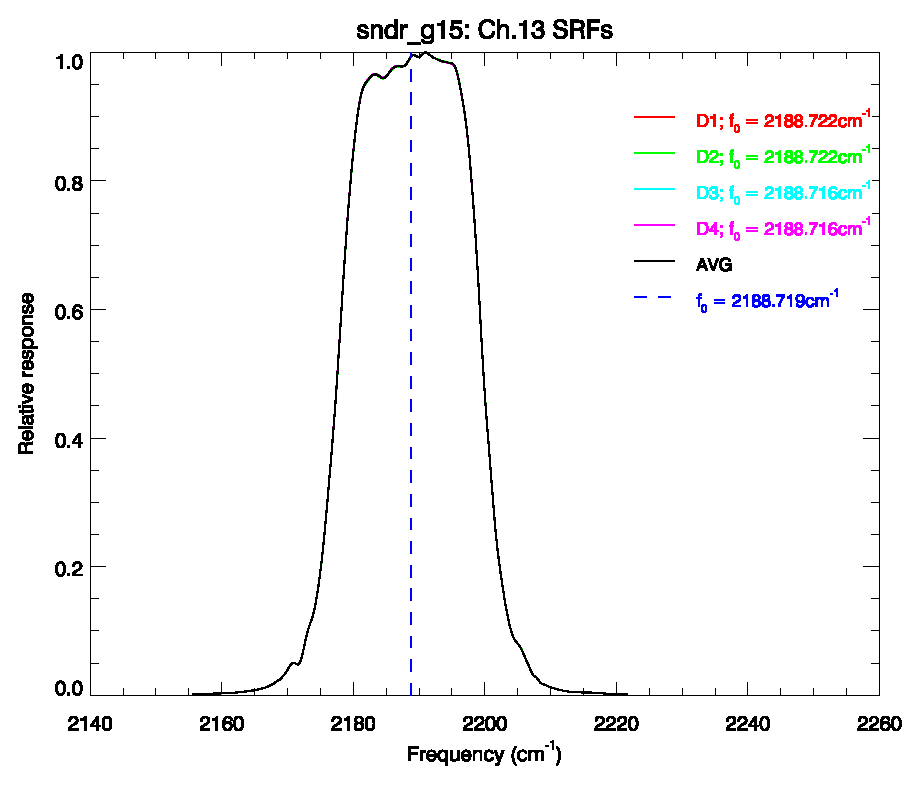
\includegraphics[scale=0.5]{graphics/nominal/sndr_g15.ch13.srf.eps} &
    \includegraphics[scale=0.5]{graphics/nominal/sndr_g15.ch14.srf.eps} \\
    \includegraphics[scale=0.5]{graphics/nominal/sndr_g15.ch15.srf.eps} &
    \includegraphics[scale=0.5]{graphics/nominal/sndr_g15.ch16.srf.eps} \\
    \includegraphics[scale=0.5]{graphics/nominal/sndr_g15.ch17.srf.eps} &
    \includegraphics[scale=0.5]{graphics/nominal/sndr_g15.ch18.srf.eps}
  \end{tabular}
  \caption{GOES-P(15) Sounder SRF for channels 13 to 18.}
  \label{fig:sndr_g15.ch13-18}
\end{figure}

\subsection{Anomalous Features}
%------------------------------
Closer inspection of the GOES-P(15) sounder SRFs showed some possible anomalies for several channels. Magnifications of the SRF plots for the suspect channels are shown in figure \ref{fig:sndr_g15.zoom_anomaly}. The anomalies in question here are,
\begin{description}
  \item[Ch.9] This is not so much an anomaly as an apparent overfit to noisy data using a spline (or high order polynomial). If the high frequency undulations are a fitting artifact, the radiometric impact is likely negligible, but they are cause for suspicion.
  \item[Ch.11] Similarly to channel 9, there appear to be fit artifacts in the data.
  \item[Ch.13] The detector plots are different. Does the GOES-P(15) sounder use different shortwave detector technology from the other sounder? Previously the InSb detector channels showed no difference between detectors. It may be a normalisation of fitted data issue, but it needs to be confirmed.
  \item[Ch.17] Similarly to channel 13, we see significant differences between detector SRFs for InSb detectors.
  \item[Ch.18] Again, we see significant differences between detector SRFs for InSb detectors.
\end{description}


\begin{figure}[htp]
  \centering
  \begin{tabular}{c c}
    \hspace{1.0em}\textsf{Spline fit of noisy data?} &
    \textsf{Spline fit of noisy data?} \\
    \includegraphics[scale=0.5]{graphics/zoom_anomaly/sndr_g15.ch9.srf.eps} &
    \includegraphics[scale=0.5]{graphics/zoom_anomaly/sndr_g15.ch11.srf.eps} \\\\
    \hspace{1.0em}\textsf{InSb detector differences?} &
    \hspace{1.0em}\textsf{InSb detector differences?} \\
    \includegraphics[scale=0.5]{graphics/zoom_anomaly/sndr_g15.ch13.srf.eps} &
    \includegraphics[scale=0.5]{graphics/zoom_anomaly/sndr_g15.ch17.srf.eps} \\\\
    \hspace{1.0em}\textsf{InSb detector differences?} & \\
    \includegraphics[scale=0.5]{graphics/zoom_anomaly/sndr_g15.ch18.srf.eps} &
  \end{tabular}
  \caption{Magnification of GOES-P(15) Sounder SRFs for channels 9, 11, 13, 17, and 18; indicating possible data anomalies. Detector and average plot colours are the same as for previous figures.}
  \label{fig:sndr_g15.zoom_anomaly}
\end{figure}
\end{document}

